\chapter{The IceCube Detector}\label{chapter:icecubedetector}
The IceCube Detector is a large (cubic kilometer scale) water cherenkov detector situated underneath the ice at the south pole. Its large volume makes it ideal for studying high energy (TeV and higher) neutrino events originating from either the atmosphere or astrophysical sources. 

\section{Detection Mechanism}
The cross section for neutrino interaction in Earth can be seen in figure \ref{fig:cross_sections}. These cross sections are small, but the Earth is also quite large. We can calculate the mean free path for neutrinos traveling through Earth as (eq. \ref{mfp}):

\begin{equation}
    \lambda = \frac{1}{\sigma_{\nu}\rho_{Earth}}
    \label{mfp}
\end{equation}

Using the neutrino cross section near 1 PeV ($\sigma_{\nu} \approx 10^{-33}$ cm$^2$), and the density of the Earth ($\approx 5.5$ g/cm$^3$, corresponding to a nucleon density of $\rho_{Earth}=3.3 \times 10^{24}$ cm$^{-3}$), we obtain an estimate of the neutrino mean free path of $\approx 3000$ km. Since the diameter of the Earth is approximately $1.3 \times 10^4$ km, we can conclude that the Earth is opaque to high energy neutrinos. We can detect the neutrinos that interacted in the Earth by way of identifying their interaction products. 

For the purposes of neutrino point source searches, we primarily focus on neutrinos interacting either through charged current (CC) or neutral current (NC) interactions. In both cases, the energy of the neutrinos observed by the IceCube detector is high enough that neutrinos interact through deep inelastic scattering with nucleons in the antarctic ice. In neutral current (NC) interactions, the process is mediated by a neutral Z boson, as shown on the left in figure \ref{fig:nuinteractions}. In this case, the product of the interaction is a neutrino, meaning the only visible signature of this interaction is the production of a hadronic particle cascade. 

\begin{figure}[h]
\centering
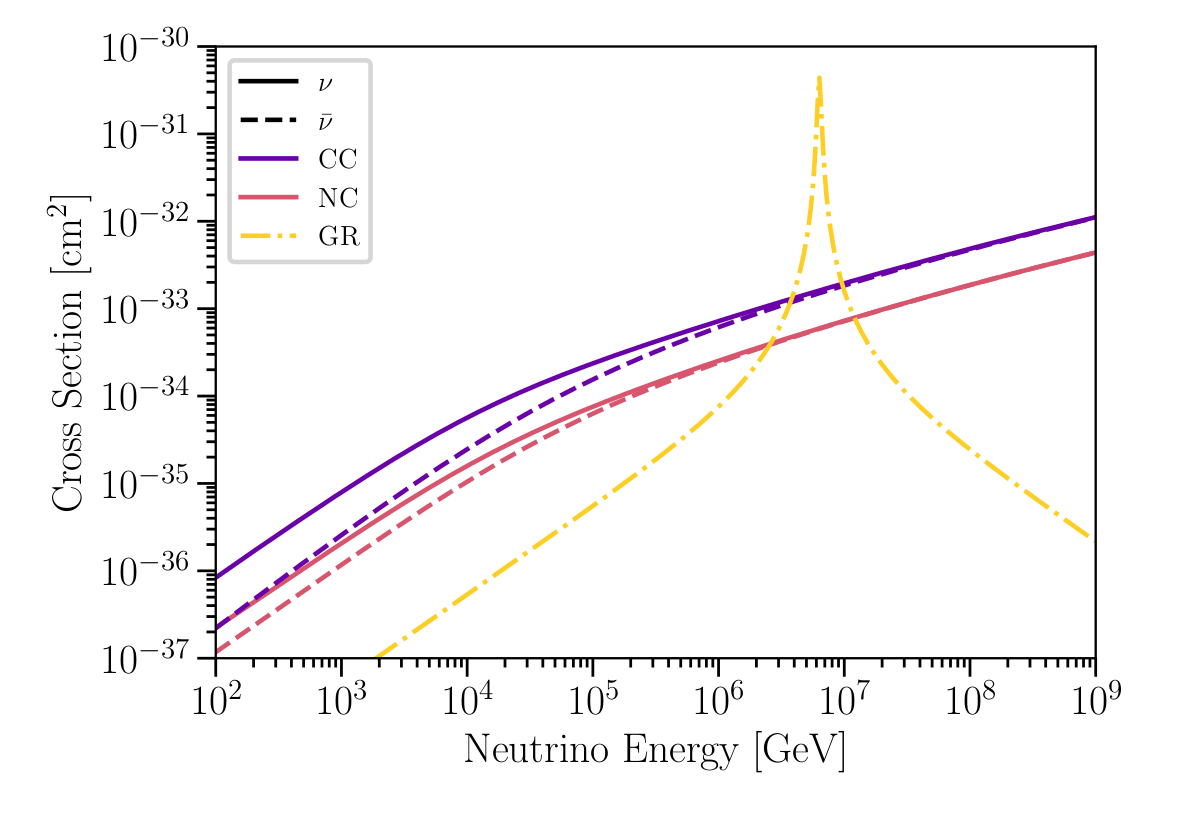
\includegraphics[width=0.8\textwidth]{figs/nu_cross_sections.png}
\caption{The cross sections of various neutrino interactions in the Earth. The yellow curve corresponds to Glashow Resonance \cite{IceCubeGlashow}, whereby an anti-electron neutrino combines with an atomic electron to produce a W+. These events are relatively rare in IceCube data, and are subsequently not used in the context of astrophysical neutrino source searches.}
\label{fig:cross_sections}
\end{figure}

Charged current interactions are mediated by a charged W boson, and can be summarized as (eq. \ref{ccinteraction1} and \ref{ccinteraction2}):

\begin{equation}
    \nu_\ell +  n \rightarrow \ell^- + p
\label{ccinteraction1}
\end{equation}
\begin{equation}
    \bar{\nu}_\ell +  p \rightarrow \ell^+ + n
\label{ccinteraction2}
\end{equation}

The Feynman diagrams for this process can be seen on the right in figure \ref{fig:nuinteractions}. Notably, charged current interactions produce an outgoing lepton $\ell^\plusminus$ in addition to a hadronic cascade. This is particularly useful in the case that the lepton produced is a muon, as muons can travel a sizeable distance (hundreds, or even thousands of meters) before decaying. If the lepton recieves enough energy, it will subsequently produce cherenkov radiation, as it will be traveling faster than the local speed of light in ice. This radiation is emitted at an angle $\theta_c$ relative to the direction of travel, where $\theta_c$ is given by (eq. \ref{cherenkoveq}):

\begin{equation}
    \cos(\theta_c) = \frac{1}{n\beta}
\label{cherenkoveq}
\end{equation}

Where $n$ is the index of refraction of the medium through which the particle is traveling (in this case ice), $\beta = \frac{v}{c}$, and $v$ is the velocity of the traveling particle (the lepton, in this case).  For ice, $n=1.31$, and this emission angle is approximately 41 degrees. The number of photons expected per unit track length is given by the Frank-Tamm formula \cite{FrankTamm} (eq. \ref{FrankTamm}):

\begin{equation}
    \frac{dN}{dxd\lambda} = \frac{2\pi z \alpha}{\lambda^2}\sin^2(\theta_c)
\label{FrankTamm}
\end{equation}

Where $z$ is the charge of the ionizing particle, $\lambda$ is the wavelength of the emitted radiation, $\alpha$ is the fine structure constant ($\approx \frac{1}{137}$), and $\theta_c$ is the cherenkov angle given by eq. \ref{cherenkoveq}. Peak emission is found in the optical portion of the light spectrum, between 350 and 600 nm corresponding to a characteristic blue hue. 

To summarize, neutrinos traveling through the antarctic ice will occasionally interact, producing child particles that will emit cherenkov radiation. We can then build an array of photon detectors to detect these photons, and subsequently infer information about the original incident particles. 

\begin{figure}[h]
\centering
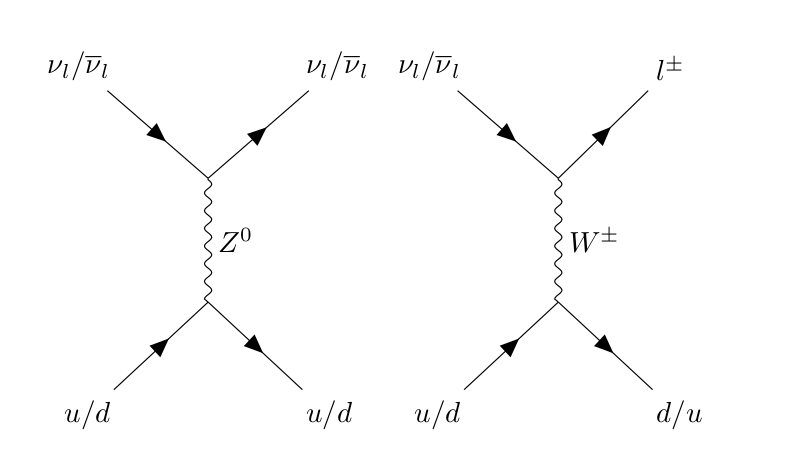
\includegraphics[width=0.8\textwidth]{figs/nuinteractions.png}
\caption{The Feynman diagrams corresponding to neutral current (left) and charged current (right) neutrino interactions. Charged current interactions can produce a detectable outgoing lepton in addition to a hadronic cascade, while neutral current interactions only produce a hadronic cascade.}
\label{fig:nuinteractions}
\end{figure}

\section{The Physical Components of the IceCube Detector}
As outlined in the previous section, the strategy for detecting neutrinos with a water cherenkov detector is not to directly detect the neutrinos themselves, but rather to detect the cherenkov photons from the outgoing particles resulting from the neutrino interactions. The IceCube detector accomplishes this through the use of a large number of photomultiplier tubes (PMTs). At the very highest level, a PMT is a device that converts photons to an electrical signal that can then be read out by a set of associated electronics. The details of general PMT design and operation can be found in \cite{tavernier_pmt}.

\begin{figure}[h]
\centering
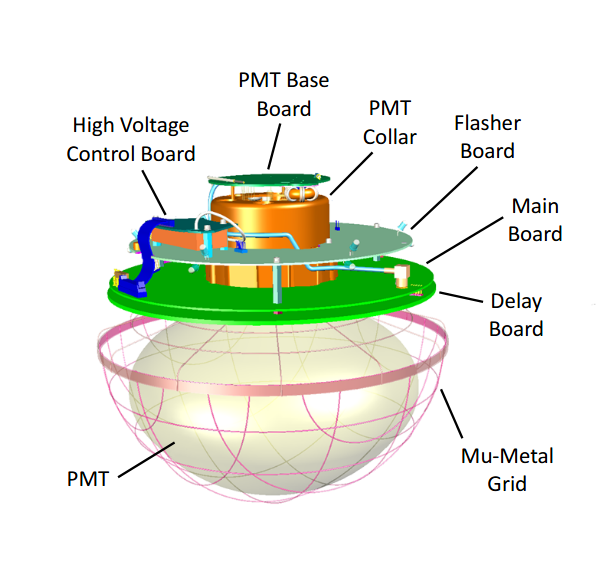
\includegraphics[width=0.8\textwidth]{figs/DOM.png}
\caption{A diagram of a single IceCube digital optical module (DOM). The entire apparatus is encased in a pressurized glass sphere for protection (not shown). The PMT faces downward for optimal collection of photons from upgoing neutrino events. In addition to the PMT, each DOM also contains digitization electronics and an array of LED flashers that can be used for calibration ~\cite{det_paper}. }
\label{fig:DOM}
\end{figure}

In IceCube, PMTs are housed in a single unit referred to as a digital optical module ("DOM"), seen in figure \ref{fig:DOM}. Each module contains the PMT and its associated electronics, as well as a set of LED flashers that can be used to calibrate the detector once the DOMs have been lowered into the ice. DOMs are arranged onto 86 vertical strings, 78 of which contain 60 DOMs spaced ~17 meters apart along the length of the string. These strings are arranged into a hexagonal grid pattern under the south pole ice with a separation between strings of approximately 125 meters, resulting in a cubic kilometer of instrumented ice extending between 1400 and 2400m below the surface of the south pole ice sheet. The remaining 8 strings form the DeepCore sub-array, a more densely instrumented region near the center of the detector, primarily used for studying lower ($\approx$100s of GeV) scale events. PMTs that are part of the DeepCore portion of the detector have a higher quantum efficiency than those on the other 78 strings \cite{deepcorepaper}.  

A diagram of the IceCube detector can be seen in figure \ref{fig:icecubediagram}. Due to the weakly interacting nature of neutrinos combined with a power law spectrum, a large detector volume is critical to detecting the astrophysical neutrino flux. Prior to IceCube's construction, calculations indicated that a cubic-kilometer scale detector would be necessary to observe an appreciable event rate of astrophysical neutrinos \cite{Halzen_2002}\cite{Waxman_1998}. The size and design of IceCube are well suited for detecting astrophysical neutrino events in the TeV+ energy range, as the large instrumented volume ensures a significant number of interactions in this energy range, and the detector's nanosecond scale timing resolution makes event reconstruction possible for events producing cherenkov radiation over the scale of $\approx$100s of meters. 

\begin{figure}[h]
\centering
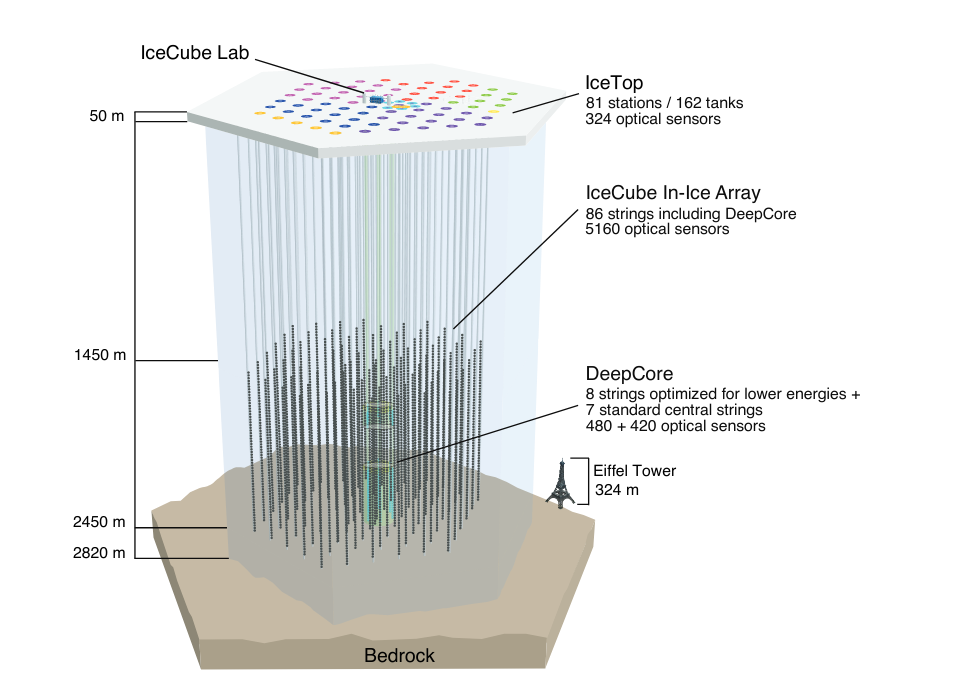
\includegraphics[width=0.8\textwidth]{figs/icdiagram.png}
\caption{A diagram of the IceCube detector. The detector consists of 86 strings of DOMs lowered into holes drilled in the pattern of a hexagonal grid defined by a separation of 125 meters. Each string is formed by 60 DOMs connected by a cable, used for powering the DOMs and communication with the IceCube Lab (ICL) on the surface. The instrumented detector volume begins at a depth of 1450 meters, and extends down to 2450 meters, resulting in approximately a cubic kilometer of instrumented ice~\cite{det_paper}. }
\label{fig:icecubediagram}
\end{figure}

As the IceCube detector is situated in the south pole ice, a proper description of the optical properties of the ice is key for being able to accurately reconstruct events. While the ice is generally clear, it does contain several impurities and features that make it optically nonuniform. The scattering and absorbtion of light are known to vary as a function of depth, as seen in figure \ref{fig:icedepth}. The large peak near a depth of 2000 meters is thought to correspond to a layer of dust deposited on the south pole ice sheet many years in the past, and is commonly referred to as "the dust layer" (physicists are not always the most creative with names). 

In addition to varying as function of depth, the optical properties of the ice also vary as a function of azimuth. The largest effects along this axis are the ice tilt and ice anisotropy. The ice tilt refers to the layers of ice with similar optical properties being not perfectly horizontal, and results in a variation in scattering and absorption as light travels in different directions through the ice sheet. The ice anisotropy is similar, but has an observed additional axis of symmetry, leading to variations that are twice as frequent as a function of azimuth. Notably, while this effect was original observed in calibration data using LED flashers, it is visible in data from observed atmospheric muons, as seen in figure \ref{fig:anisotropyplot}. 

The final major optical nonuniformity of the detector ice is the hole ice. During the construction of the IceCube detector, holes were drilled in the south pole ice, and strings of DOMs were lowered down the appropriate depth. The water in these holes then refroze with different optical properties than the surrounding ice. The column of refrozen ice is referred to as the "hole ice", typically containing an inner region where air bubbles have been trapped referred to as the "bubble column". The hole ice has significantly shorter scattering distances, and is an area of active study within the IceCube collaboration. 

\begin{figure}[h]
\centering
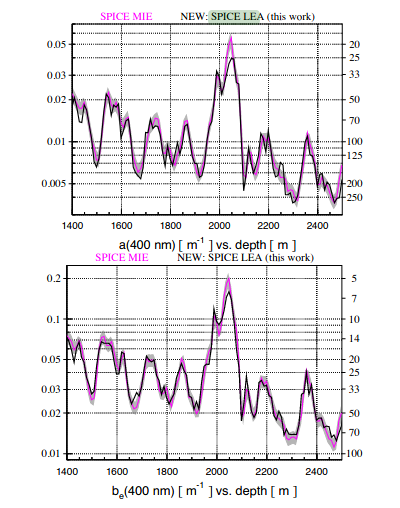
\includegraphics[width=0.8\textwidth]{figs/icedepth.png}
\caption{Plots of the scattering and aborption of light as a function of depth in the south pole ice. The peak near a depth of 2000 meters is referred to as "the dust layer", and is thought to correspond to a layer of dust deposited at the south pole at some point in the Earth's history.  ~\cite{iceproceedings} }
\label{fig:icedepth}
\end{figure}

\begin{figure}[h]
\centering
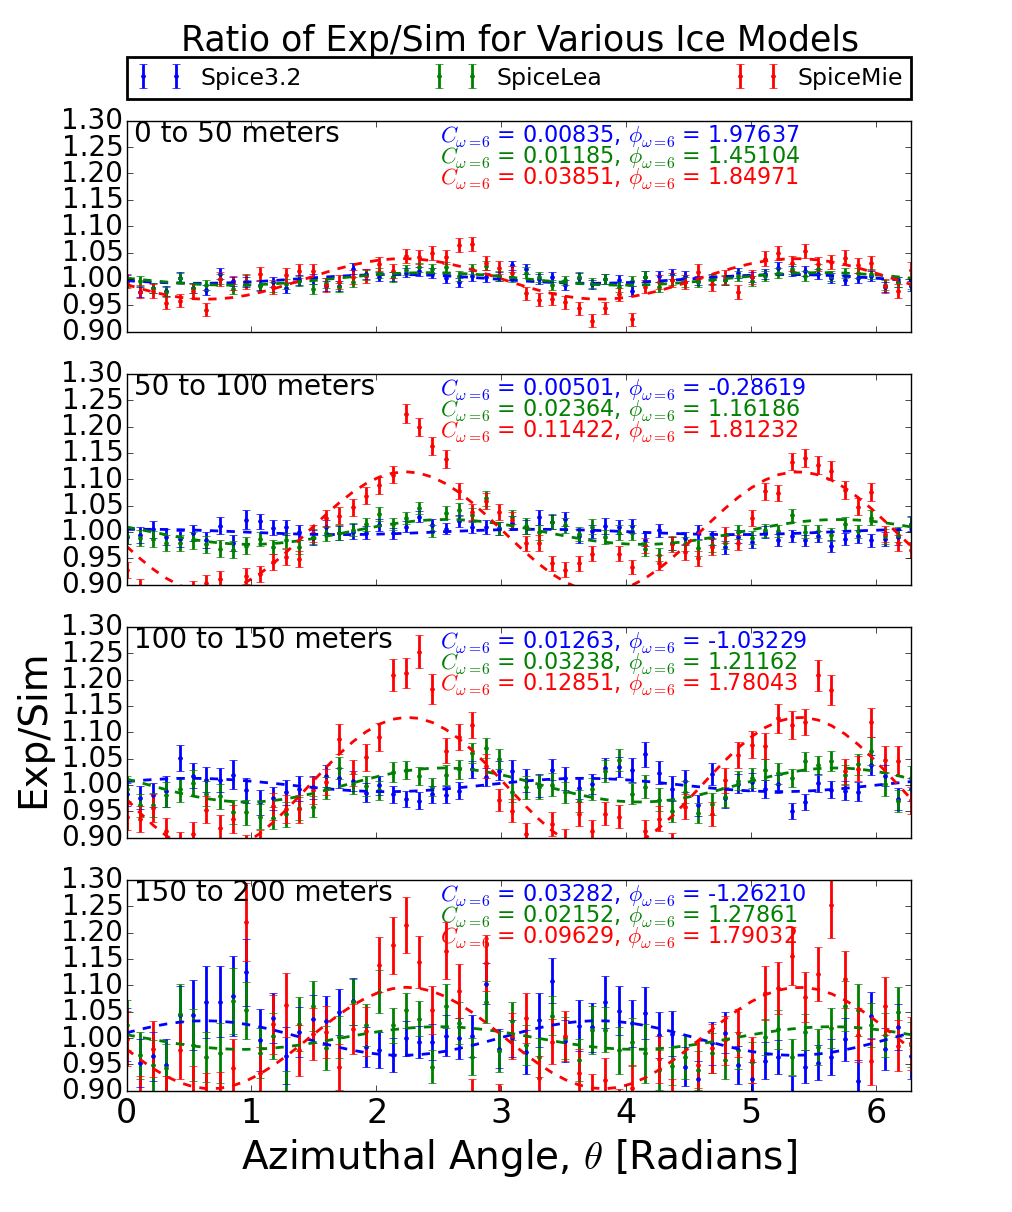
\includegraphics[width=0.8\textwidth]{figs/fourierfits.png}
\caption{Plots of the ratio of light seen from atmospheric muons in experiment and simulation using various ice models (SpiceMie, SpiceLea, and Spice3.2), as a function of azimuthal angle between the muon track and the observing DOM. SpiceMie does not account for the ice anisotropy, resulting in a sinusoidal shape that grows with distance. SpiceLea and Spice3.2 both account for the anisotropy, and consequently the sinusoidal shape is reduced in amplitude when using these ice models.}
\label{fig:anisotropyplot}
\end{figure}

\section{Event Types}
IceCube events can be generally be categorized into three different types: tracks, cascades, and double cascades. While neutral current events exclusively correspond to cascades, charged current events can produce any of the three, dependent on the variety of the outgoing lepton. This gives IceCube the ability to identify the flavor of the incident neutrino, and this fact can be leveraged to do a large amount of interesting physics. However, for the purposes of this work, we are primarily interested in tracks, due to their excellent pointing resolution as discussed below. 

\subsection{Tracks}
From equation \ref{ccinteraction1} we can see that charged current interactions produce an outgoing lepton, which will in turn produce cherenkov radiation if it is energetic enough. In particular, if the outgoing particle is a muon, it will travel a significant distance before decaying or exiting the detector. As the muon produces cherenkov radiation as it travels through the ice, the pattern of DOMs which detect this radiation will resemble a line, as shown in figure \ref{fig:evttypes}. These events are referred to as "tracks". If the neutrino interaction occurred inside the IceCube detector, then the track will appear to start within the detector, and the event can be referred to as a "starting track". If instead the neutrino interaction occurred outside the detector, and the resultant muon traveled through the detector, then the event is instead referred to as a "through-going track" (again, physicists are not the most creative). Through-going tracks can result from astrophysical neutrinos, as well as atmospheric neutrinos and atmospheric muons (muons resulting from cosmic ray interactions in the atmosphere). Starting tracks, however, can only be produced by muons originating from atmospheric or astrophysical neutrinos. For the purposes of this work, we will focus primarily on through-going tracks, however starting tracks are also scientifically interesting, and can be used for point-source and diffuse analyses of the neutrino flux as well \cite{Estes}.

\begin{figure}[h]
\centering
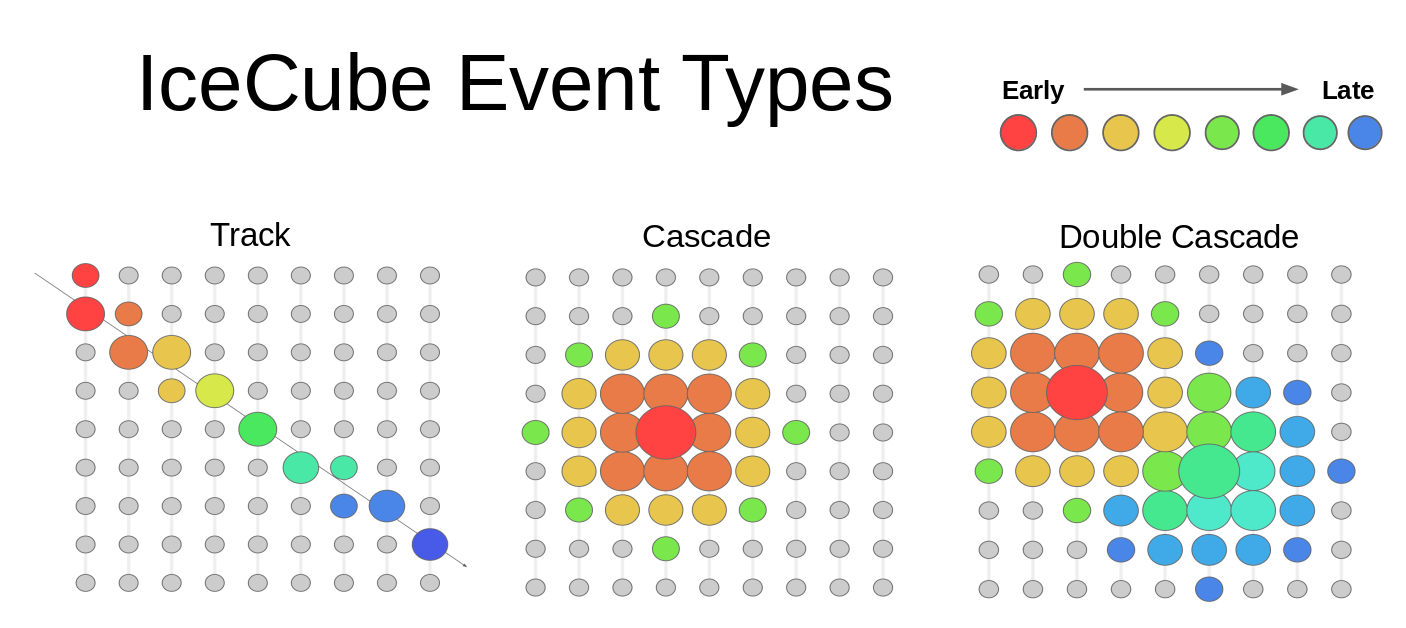
\includegraphics[width=0.8\textwidth]{figs/evt_types.png}
\caption{Cartoons in the x/z plane depicting the various event types seen by the IceCube detector. Grey circles are intended to represent individual DOMs, while colored circles correspond to DOMs that saw photoelectrons. The size of the circle corresponds to the amount of charge seen, while the color denotes the timing. Of most relevance to this work are tracks (left), as their long lever arm provides good pointing resolution.}
\label{fig:evttypes}
\end{figure}


Through-going tracks are notable for their good angular resolution ($<$ 1 degree), particularly at high energies ($> 1$ TeV), as seen in figure \ref{fig:angres}. This makes them an excellent candidate for attempting to do astronomy, as the can be expected to point back to their point of origin with reasonable accuracy. Energy reconstruction of these events is somewhat more challenging, however, due to a combination of stochastic energy losses of the muon producing the cherenkov photons, and the fact that the event itself is often not entirely contained in the detector. The energy resolution of tracks in IceCube is approximately a factor of 2 at 10 TeV, though this increases for higher energy events \cite{10yrpublicdata}.

\begin{figure}[h]
\centering
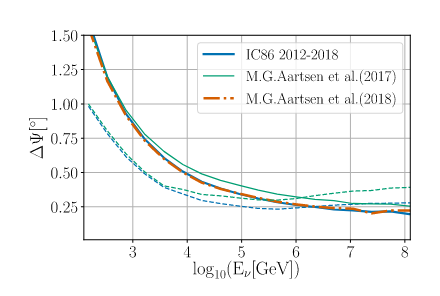
\includegraphics[width=0.8\textwidth]{figs/angres.png}
\caption{The median angle between simulated neutrino and reconstructed muon directions as a function of energy for various high-statistics IceCube samples composed of track events. The dark blue line corresponds to PSTracks v003p02, the light blue line corresponds to PSTracks v002p03, and the orange dashed line corresponds to NorthernTracks v002p06 (see section 1.7 for a description of these data samples). The solid lines describe events in the northern hemisphere, while the dashed lines are events in the southern hemisphere \cite{10yr_tint}\cite{NorthernTracks_PS}\cite{7yr_tint}.}
\label{fig:angres}
\end{figure}

\subsection{Cascades}
In CC interactions, the initial interaction produces a hadronic cascade regardless of the variety of outgoing lepton produced. If the outgoing lepton is an electron, the interaction length is relatively short, typically less than the 125 meter spacing of IceCube strings. Because of this, the resultant pattern of DOM hits in the detector is formed from the combined hadronic and electromagnetic showers. As the two showers occur at approximately the same spatial position, this appears to the detector as a single cascade. While due to their spherical symmetry cascades tend to have poor (10 degree or more) pointing resolution, they have excellent energy resolution, as even for high energy events, the entirety of the cascade is often contained within the detector, making energy reconstruction as simple as counting the total number of cherenkov photons produced. The energy resolution of cascades is approximately 15\%, potentially even lower at higher energies \cite{AustinThesis}.

\subsection{Double Cascades}
If the outgoing lepton from a CC interaction is a tau, then it may travel a relatively short distance before interacting again. If the initial tau is high enough energy, this can produce a signature of two spatially separated hadronic cascades in the detector. If the tau is lower energy, the two cascades may not be spatially resolvable, though may still be able to be identified by examining the waveforms observed by hit DOMs. This type of event was only recently observed in IceCube data \cite{taupaper}. Notably, tau events of these energies are not expected to be produced by atmospheric processes, and consequently this observation provides further evidence of an astrophysical neutrino flux. 

\section{Triggering}
IceCube DOMs are subject to dark noise in the detector originating from PMTs emitting electrons from the cathode in the absence of an external photoelectron. This noise should not be correlated between nearby DOMs, and can be dramatically reduced by imposing the triggering requirement that neighboring DOMs also experience a signal with $\plusminus$ 1 $\mu s$. These hits are classified as "Hard Local Coincidence" (HLC). An eight-channel simple majority trigger (SMT8) is used to trigger a readout window where DOM information is written to file. This trigger requires eight DOMs to have HLC hits within a 5 $\mu$s window. 

Events are further filtered through several additional algorithms to pare down events based on temporal and spatial coincidence of DOM hits. The result is a "Level 2" event rate of approximately 2.5 kHz. These events can be additionally filtered to select specifically for high quality track-like events (originating mostly from atmospheric muons, but also from atmospheric and astrophysical muon neutrinos as well), reducing the event rate to ~Hz. This level of data is often referred to within the collaboration as "Muon Level 3", and primarily consists of through-going track-like events. 

\section{Directional Reconstruction}
In this section we discuss algorithms for reconstructing the direction of through-going track events observed by the IceCube detector. Different algorithms may be used for cascades, though understanding these is unimportant for the remaining content of this thesis. Those who are interested in the reconstruction of cascade and double cascade events can refer to \cite{AustinThesis}.

\subsection{LineFit}
An initial guess for the reconstructed direction of the track can be obtained by ignoring the geometry of the cherenkov cone and the optical properties of the ice, and assuming a plane wave of light traveling along a straight line in the detector. The location of each DOM that observes photons ($\textbf r_i$) can then be written as a line (eq. \ref{linefit1}):

\begin{equation}
    \textbf r_i = \textbf r + \textbf v \cdot t_i
    \label{linefit1}
\end{equation}

Where $t_i$ is the time that the $i$th DOM observes photons, \textbf{r} is the vertex of the track, and \textbf{v} is the velocity of light in the ice. A $\chi^2$ fit can then be preformed to determine the free parameters \textbf{r} and \textbf{v} (eq. \ref{linefit2}):

\begin{equation}
    \chi^2 \equiv \sum_{i=1}^{N_{tot}}(\textbf r_i - \textbf r - \textbf v \cdot t_i)^2
    \label{linefit2}
\end{equation}

This can be solved analytically, resulting in fitted vectors for \textbf{r} and \textbf{v} (eq. \ref{linefit3} and \ref{linefit4}):

\begin{equation}
    \textbf r = \langle \textbf r_i \rangle - \textbf v \cdot \langle t_i \rangle
    \label{linefit3}
\end{equation}

\begin{equation}
    \textbf v = \frac{\langle \textbf r_i \cdot t_i \rangle - \langle \textbf r_i \rangle \cdot \langle t_i \rangle }{\langle t_i^2 \rangle - \langle t_i \rangle^2}
    \label{linefit4}
\end{equation}

This corresponds to a vertex (\textbf{r}) and a direction (\textbf{v}) describing the path of the particle. Further discussion on this topic can be found in \cite{track_reco_paper}.

\subsection{SplineMPE}
An improved reconstruction of the particle direction can be obtained by iterating on the initial LineFit reconstruction described above. The LineFit result is treated as a seed for a likelihood based reconstruction that takes the cherenkov angle and ice properties into account. A description of the specific likelihood components may be found in section 3 of \cite{track_reco_paper}. In the simplest implementation of this likelihood method, only information from the first photoelectron observed by a particular DOM is used. This is referred to as a single photoelectron fit, or "SPEFit". For events that produce multiple hits on a single DOM, this information can be included in the likelihood as well, producing a multi-photoelectron (MPE) fit. Since photons arriving after the first are likely to have experienced at least some scattering, a proper description of the ice properties is necessary for an accurate MPE fit. This is incorporated into the likelihood described in \cite{track_reco_paper} via the use of tabulated timing and light yield distributions for various DOM/photon configurations given an ice model developed from fits to LED flasher data \cite{icemodel_paper}. The information in these tables is stored via a multi-dimensional spline, allowing these tables to be used directly as PDFs in the MPE likelihood, hence the name for this variety of reconstruction: "SplineMPE".

\subsection{Paraboloid}
There is some inherent uncertainty associated with the observation and reconstruction of a particular event. For an event originating from a particular true position, the reconstructed position is expected to be drawn from distribution centered on the true position. Properly describing this distribution is key to characterizing the per-event uncertainty associated with the directional reconstruction, and is important for obtaining accurate results in a point source analysis.

A semi-analytic description of the angular error associated with a particular event can be obtained from the likelihood map associated with the direction reconstruction outlined in the previous section. An ellipse can be fit around the global minimum of the likelihood map, describing a $1 \sigma$ containment region. The ellipse is parameterized by two variables, $\sigma_1$ and $\sigma_2$ describing the scales of the two axes of the ellipse, and an average circularized error can be computed as (eq. \ref{circerr})\cite{paraboloidpaper}:

\begin{equation}
    \sigma_{evt} = \sqrt{\frac{\sigma_1^2 + \sigma_2^2}{2}}
\label{circerr}
\end{equation}

This description can be further improved by comparing this error with the "true error" obtained from examining the difference between the simulated event direction and the corresponding reconstructed direction. By multiplying the above circularized error by the ratio of the reconstructed error to the "true" error, we remove potential bias due to effects not accounted for by the directional reconstruction algorithm. For example, one such effect would be the angle between the incident neutrino and the outgoing muon. Since the reconstruction algorithm only reconstructs the direction of the track associated with the muon, the direction of the neutrino is still technically unknown. While at high energies the muon and it's parent neutrino can be assumed to be colinear, this angle becomes a significant source of uncertainty below 1 TeV. 

\section{Energy Reconstruction}
While the direction of track event in IceCube can be reconstructed with good precision using the methods described previously, reconstructing the energy is more difficult. The primary reason for this is simply a lack of information: since many tracks originate from events neutrino interactions outside of the instrumented volume, the entirety of the muon track is not contained within the detector. This prevents the detector from behaving as a calorimeter, and estimates must be made to extrapolate the initial event energy based on the portion of the track observed. Similar to the directional reconstruction, an energy reconstruction of a particular event can be obtained using a likelihood based approach based on the individual DOM observations. 

At its core, this likelihood approach assumes that the number of detected photoelectrons ($k$) is expected to be poisson distributed with a mean directly proportional to the energy: $\lambda=E \Lambda$ (eq. \ref{erecolh}), where $\Lambda$ is the number of photons the event produces per unit energy:

\begin{equation}
    \mathcal{L} = \frac{(E \Lambda)^k}{k!} e ^ {-E \Lambda}
\label{erecolh}
\end{equation}

Maximizing this likelihood over all $j$ DOMs that see photoelectrons results in the relation (eq. \ref{erecoeq}):

\begin{equation}
    E = \sum{k_j}/\sum{\Lambda_j}
\label{erecoeq}
\end{equation}

Which is largely a statement that the event energy is proportional to the number of observed photons, scaled by some factor that is the sum of the light yield scaling functions $\Lambda_j$. These functions depend on a variety of factors including the geometry and ice optical properties. Much like in the case of the directional reconstruction, these functions are often obtained from tabulated monte carlo data, smoothed with a multi-dimensional spline. 

This likelihood can then be applied to calculate the energy loss rate ($\langle dE/dx \rangle$) of a particular muon. Above 1 TeV, this energy loss rate is roughly proportional to the muon energy. A robust estimate of this rate can be obtained by fitting segmented energy losses along the muon track using the methodology described in \cite{erecopaper}. Once a list of segmented energy losses is calculated, there are several different approaches to converting to a reconstructed energy. 

\begin{itemize}
    \item \textbf{MuEX} takes the average of the segmented energy losses and uses that as an estimate of the energy
    \item \textbf{TruncatedEnergy} first removes the largest 40\% of energy losses before calculating an average, ideally reducing the variance in the calculation of $\langle dE/dx \rangle$. 
\end{itemize}

A comparison of these approaches can be found in \cite{erecopaper}, and both methods provide approximately 35\% precision in $\log_{10}E$ for an initial muon energy of $10^4$ GeV, improving slightly to approximately 30\% in $\log_{10}E$ at higher energies. 

\section{IceCube Event Samples Overview}
As the Icecube detector is capable of doing a wide variety of science, there exists a plethora of event samples used within the collaboration. Even within the context of searches for point sources of astrophysical neutrinos, there exist several event samples of IceCube events, each with their own selection criterion and set of reconstructed parameters. In many cases, the distinguishing features between event selections used in point source analyses are purity and event rate. An ideal point source event sample would have both a high purity of astrophysical events in addition to a high event rate. Unfortunately, this is not possible with the current iteration of the IceCube data, as we observe relatively few events above 100 TeV (where the highest purity of astrophysical events can be achieved), and below 100 TeV there is a significant irreducible background of atmospheric neutrinos. 

For this reason, point source event samples in the IceCube collaboration generally follow two different philosophies. "Low statistics/high purity" samples contain relatively few events, but the events in these samples have a high probability of being astrophysical in origin \cite{Estes} \cite{hese7yr}. By contrast "high statistics/low purity" samples contain a higher number of events, including additional astrophysical events. However in doing so, these samples also include significantly more atmospheric (background) events \cite{stettner2019measurement} \cite{10yr_tint}. In the context of point source searches, these samples typically rely on advanced statistical methods in their analysis pipeline to distinguish between clustered astrophysical signal and isotropic atmospheric background. 

Even within the category of high statistics/low purity samples used for neutrino source searches, there exist multiple samples that are regularly used within the IceCube collaboration. The following sections will briefly outline three such samples that are relevant to the analyses presented later in this work.  

\subsection{PointSourceTracks v002p03}
Starting with Muon level 3 data, this sample applies an additional BDT to attempt to select for well-reconstructed muon neutrino interactions from mis-reconstructed atmospheric muon background. The variables used in this BDT were associated with a track-like event topology, and the BDT was trained using both background data, as well as simulation of both an $E^{-2.0}$ and $E^{-2.7}$ signal. The result is a high-statistics sample of mostly track-like neutrino events in the northern sky, consisting of both atmospheric and astrophysical neutrinos \cite{7yr_tint}. Events in this sample use a SplineMPE reconstruction ("plain" settings, corresponding to a balance of computation time and precision) for the event direction, and a MuEX reconstruction for the event energy.


This sample covers seven years of IceCube data (2008-2015), and was used for the historical untriggered flare analysis of TXS0506+056 \cite{TXS_Archival}, where a $3.5\sigma$ neutrino flare was identified in 2014. 

\subsection{PointSourceTracks v003p02}
Though this sample is oftentimes treated as a "successor" to PointSourceTracks v002p03, it is in many ways a completely new event selection. This sample covers 10 years (2008-2018) of IceCube data. Like v002p03, this sample also starts with Muon level 3 data, however here the BDT is trained to additionally reject cascade-like events in addition to accepting track-like events. Additionally, an improved directional reconstruction is used: the SplineMPE reconstruction algorithm is applied twice, with the second application using the results of the first as a seed, and additionally including the energy estimation. This results in improved angular resolution \cite{TessaThesis}.

This sample additionally requires that events pass some precuts prior the the application of the BDT. Events are only selected if they satisfy the conditions below:

\begin{itemize}
    \item The length of empty track (the portion of the reconstructed track that does not have any associated DOM hits) must be $\leq 400$m
    \item The reconstructed track length must be at least 200m
    \item The number of hit DOMs must be $\geq 12$
    \item The number of DOMs that observe direct (non-scattered) photons must be $\geq 6$
    \item $\cos(\theta_{geo}^2) < 0.2$, where $\theta_{geo}$ is the angle between independent reconstructions calculated for the first and second half of the track only. For a high quality track, both the first half reconstruction and the second half reconstruction should lie almost parallel. 
\end{itemize}

This sample also has different requirements for events observed from the southern sky. The minimum track length and maximum empty track length pre-cuts are applied as in the northern sky, in addition to an additional cut that the initial estimated uncertainty ($\sigma_{paraboloid})$ must be less than 5 degrees. A cut on the likelihood reconstructions is also enforced, requiring $R\log(\mathcal{L}) > 9$, where $R\log(\mathcal{L}$ is the "reduced log likelihood", where the maximum likelihood value, $\mathcal{L}$ is divided by the number of degrees of freedom, $n_{dof}$ ($n_{dof} = 5$ in this particular case). Events in the southern sky are also required to have hits on more than 5 different IceCube strings if the number of direct DOM hits was fewer than 12 \cite{TessaThesis}. 

This sample is notable as it was the sample used for the 10-year all-sky IceCube time integrated analysis, where NGC 1068 was identified as having a significance of $3 \sigma$~\cite{10yr_tint}. This sample has also been publicly released for use outside the IceCube collaboration \cite{10yrpublicdata}.

\subsection{NorthernTracks v002p06}
The NorthernTracks sample is a high statistics, low purity sample of through-going tracks that was originally developed for the purpose of performing a diffuse fit of the atmospheric and astrophysical neutrino spectrum. As such, this sample has relatively good data/MC agreement (as this is essential to the diffuse fit analysis pipeline), but is restricted to only events in the northern sky. Additionally, this sample does not make use of data from DeepCore DOMs,  a decision that was made in order to homogenize the detector. This sample covers 8 years of livetime (2009-2017) has been used for point source analyses as well as diffuse studies of the neutrino spectrum \cite{NorthernTracks_PS}. 

The precuts for this sample in the northern sky are identical to PointSourceTracks v003p02, however this selection then uses two separate BDTs to further filter events: one BDT to select for track-like events, and a separate BDT to reject cascade-like events. In practice the application of these two BDTs is similar, but not perfectly identical, to the application of the single BDT in PointSourceTracks v003p02. Also of note is that the BDTs used in the NorthernTracks selection are trained exclusively using simulation, for both signal and background.

This sample uses a SplineMPE directional reconstruction (with "max" settings, prioritizing precision over computation speed), and a TruncatedEnergy estimator as the energy reconstruction. 

A comparison of the three samples outlined here can be seen in table \ref{tab:evtsamples}

\begin{sidewaystable}
\centering
\begin{tabular*}{0.865\textwidth}{|c|ccc|} 
\hline
. & PSTracks v2 & PSTracks v3 & NorthernTracks\\
\hline\hline
Pre-cuts & No & Yes & Yes\\ 
BDT 1 & Selects tracks & Selects tracks and rejects cascades & Selects tracks \\
BDT 2 & None & None & Rejects cascades \\
Signal training set & Simulation & Simulation & Simulation \\
Background training set & Data & Data & Simulation \\
Direction reconstruction & SplineMPE ("plain") & SplineMPE ("plain")$\times$ 2 & SplineMPE ("max") \\
Angular error estimator & Paraboloid & Paraboloid & Paraboloid \\
Energy estimator & MuEX & MuEX & TruncatedEnergy \\ 
DeepCore included? & Yes & Yes & No \\
Livetime & 7 years (2008-2015) & 10 years (2008-2018) & 8 years (2009-2017) \\
\hline
\end{tabular*}
\label{tab:evtsamples}
\caption{A comparison of several similar high statistics/low purity event samples used by the IceCube collaboration}
\end{sidewaystable}

